\section{Symmetrien}
Können in einem Graphen zwei Knoten miteinander vertauscht werden, ohne dass sich der Graph verändert, liegt eine Permutationssymmetrie vor. Für die betrachteten Netzwerke bedeutet dies, dass sich bei Vorliegen einer Permutationssymmetrie zwei Knoten tauschen lassen, indem sowohl die zugehörigen Spalten als auch Zeilen der Kopplungsmatrix getauscht werden, ohne dass sich die Dynamik des Systems verändert. Die Vertauschung der Knoten lässt sich durch eine Permutationsmatrix $P$ darstellen. Vorraussetzung für eine Permutationssymmetrie ist somit
\begin{equation}
PAP^{-1}=A.
\end{equation}

Zur Untersuchung eines Netzwerkes auf Symmetrien eignet sich die Suche von Automorphismen des dem Netzwerk zugrunde liegenden Graphen mit Hilfe der Bibliothek \textit{nauty} \cite{nauty}. Mit dieser lassen sich neben den Generatoren der Permutationssymmetrien auch die Orbits der Knoten bestimmen. Als Orbit werden hierbei die Positionen bezeichnet, an die ein Knoten durch Anwendung aller Permutationen gelangen kann. Alle Knoten eines Orbits lassen sich folglich durch eine Hintereinaderreihung der Permutationen vertauschen, ohne dass sich die Dynamik des Netzwerkes verändert. Eine solche Gruppe von Knoten wird als Cluster bezeichnet. Sollte bei der für die Vertauschung nötigen Hintereinanderreihung von Permutationen ebenfalls Knoten eines weiteren Clusters miteinander vertauscht werden, so liegt eine Verschränkung der Cluster vor (Pecora\citep{pecora2014} \textit{"interwinded Clusters"}).

\section{Synchronisation in symmetrischen Netzwerken}
Da Knoten eines Clusters ohne Veränderung der Dynamik vertauschbar sind, erhalten diese den gleichen Input der anderen Knoten und können synchron laufen. In einem aus M Clustern $C_m$ bestehenden Netzwerk existieren somit M Gruppen von Knoten, die isolierte Synchronisation aufweisen können mit synchronen Orbits $s_m$
\begin{equation}
x_i(t)=s_m(t) \text{ mit } \textit{Knoten } i\in C_m.
\end{equation}

{\subsection*{isolierte Desynchronisation}}
In einem symmetrischen Netzwerk können einzelne Cluster synchron sein, während andere nicht synchron sind. Die Desynchronisation scheint also die Synchronisation eines anderen Clusters nicht zwangsläufig zu stören.

Unter einer Permutation $\pi$ eines Clusters A mit Permutationsmatrix $P_A$ ändert sich die Dynamik eines Knotens $i$ aus einem disjunkten Cluster B nicht, es gilt



\begin{align}
		\notag \left[\boldsymbol{P}_A	\overset{\cdot}{\boldsymbol{X}}\right]_i&= \overset{\cdot}{\boldsymbol{x}}_i\\
		\notag\left[\boldsymbol{P}_A \boldsymbol{F}(\boldsymbol{X})\right]_i+
			\left[\boldsymbol{P}_A\boldsymbol{A}\boldsymbol{H}(\boldsymbol{X})\right]_i&=
			\boldsymbol{f}(\boldsymbol{x}_i)+
			\sigma\sum_j A_{ij}\boldsymbol{h}(\boldsymbol{x}_j)\\
		\boldsymbol{f}(\boldsymbol{x}_i)+
			\sigma\sum_j A_{ij}\boldsymbol{h}(\boldsymbol{x}_{\pi\left(j\right)})&=
		\boldsymbol{f}(\boldsymbol{x}_i)+
			\sigma\sum_j A_{ij}\boldsymbol{h}(\boldsymbol{x}_j)		
\end{align}
Folglich muss jeder Knoten in A gleich an den Knoten $i$ gekoppelt sein und dieser somit gleichstarken Input von allen Knoten aus A erhalten (siehe Abb. \ref{fig:perma}).

\begin{figure}
		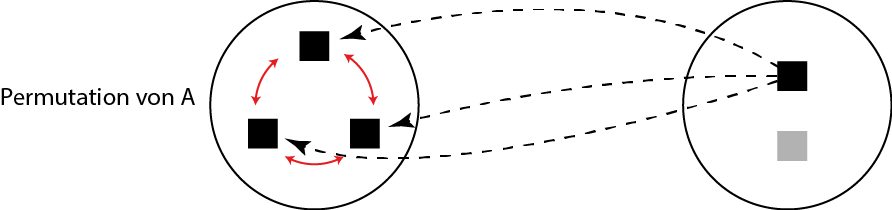
\includegraphics[width=0.75\textwidth]{abb/misc/perm_a.png}
		\caption{Es werden zwei Cluster A und B betrachtet. Eine Symmetriepermutation des Clusters A ändert die Dynamik eines Knotens in B nicht. Folglich muss dieser Knoten gleichstarken Input von jedem Knoten aus A erhalten.}
		\label{fig:perma}
\end{figure}


Eine analoge Betrachtung  unter Permutation des den Knoten $i$ enthaltenden Clusters B (A wird nicht verändert) führt auf die Beobachtung, dass jeder Knoten aus B gleich an die Knoten aus A gekoppelt ist (siehe Abb. \ref{fig:permb}). 

Zusammen ergibt sich aus diesen Aussagen: Jeder Knoten in B bekommt in der Summe den gleichen Input vom Cluster A, egal ob dieser synchron oder asynchron ist, sofern Permutationsmatrizen existieren, die die Cluster getrennt permutieren. Isolierte Desynchronisation kann nicht bei "verschränkten" Clustern auftreten, da die Permutation beide Cluster verändert.

	\begin{figure}
		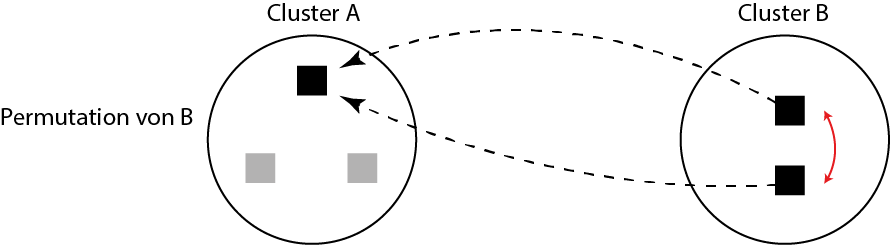
\includegraphics[width=0.75\textwidth]{abb/misc/perm_b.png}
		\caption{Bei Symmetriepermutation des Clusters B ändert sich die Dynamik eines Knotens aus B nicht. Somit muss jeder Knoten aus B gleichstarken Input von A erhalten.}
		\label{fig:permb}
	\end{figure}
	

\subsection*{Stabilität}
\label{stabilitaet}
Zur Betrachtung der Stabilität der isolierten Synchronisation lässt sich die MSE (Gleichung \ref{eq:mse})  unter Verwendung von Clustermatrizen $\boldsymbol{E^m}$ (beschreiben die Zuordnung der Knoten zu den Clustern)
\begin{align}
 \boldsymbol{E}^{(m)}_{ii} =1\text{ wenn Knoten }i \in C_m.
\end{align}
 umschreiben zu:
\begin{align}
	\label{eq:clustermse}
\notag	\delta\overset{\cdot}{\boldsymbol{X}}(t)&=	
	\left[D\boldsymbol{F}(\boldsymbol{s}(t))+\sigma\boldsymbol{A}\otimes D\boldsymbol{H}(\boldsymbol{s}(t))\right]\delta\boldsymbol{X}(t)\\&=
	\left[\sum_{m=1}^{M} \boldsymbol{E}^{(m)} \otimes D\boldsymbol{F}(\boldsymbol{s}_m(t))+\sigma\boldsymbol{A}\otimes \boldsymbol{I}_n\sum_{m=1}^{M} 			\boldsymbol{E}^{(m)}\otimes D\boldsymbol{H}(\boldsymbol{s}_m(t))\right]\boldsymbol{X}(t)
	\end{align}
	
Gleichung \ref{eq:clustermse} lässt sich unter Verwendung der Gruppentheorie in eine neue Basis transformieren. Hierbei wird die Basis der irreduziblen Darstellungen (IRRs) der den Permutationssymmetrien zugrundeliegenden Gruppe gewählt. In dieser Basis nimmt die Kopplungsmatrix Blockdiagonalform an. Die oberen M Koordinaten $\eta(t)$ in der neuen Darstellung entsprechen einer Bewegung longitudinal innerhalb der Synchronisationsmannigfaltigkeit, die weiteren einer Bewegung transversal zur ihr. Die Transformationsmatrix $\boldsymbol{T}$ lässt sich mithilfe einer geeigneten Software für diskrete Mathematik (z.B. sage) bestimmen \citep{sagenotebook}. Diese Basistransformation entspricht einer einer Transformation in $M$ Schwerpunktkoordinaten und $(N-M)$ Relativkoordinaten (die die Abweichung der Knoten eines Clusters zueinander beschreiben) mit orthogonalen Basisvektoren.

Aus der so transformierten MSE (Gleichung \ref{eq:irrmse}) lässt sich die MSF berechnen um die Stabilität der Clustersynchronisation zu beurteilen.
\begin{align}
	\label{eq:irrmse}
		\overset{\cdot}{\boldsymbol{\eta}}(t)&=
				\left[\sum_{m=1}^{M} \boldsymbol{J}^{(m)} \otimes D\boldsymbol{F}(\boldsymbol{s}_m(t))+\sigma\boldsymbol{B}\otimes \boldsymbol{I}_n\sum_{m=1}^{M} \boldsymbol{J}^{(m)}\otimes D\boldsymbol{H}(\boldsymbol{s}_m(t))\right]\boldsymbol{\eta}(t)
		\end{align}
		mit der transformierten Kopplungsmatrix $\boldsymbol{B}$ und den transformierten Clustermatrizen $\boldsymbol{J}^{(m}$
		\begin{align}
				 \boldsymbol{\eta}(t)&=\boldsymbol{T}\otimes\boldsymbol{I}_n\delta\boldsymbol{X}(t)
				\\\notag \boldsymbol{B}&=\boldsymbol{T}\boldsymbol{A}\boldsymbol{T}^{-1}
				\\\notag \boldsymbol{J}^{(m)}&=\boldsymbol{T}\boldsymbol{E}^{(m)}\boldsymbol{T}^{-1}.
		\end{align}
		




